\documentclass{article}
\usepackage[utf8]{inputenc}
\usepackage{amsmath}
\usepackage{amssymb}
\usepackage{wasysym}
\usepackage{geometry}
\usepackage{tikz}
\usetikzlibrary{shapes,arrows,positioning}
\usepackage{varwidth}
\tikzstyle{block} = [draw, rectangle, minimum height=3em, minimum width=3em]


\geometry{
 a4paper,
 total={170mm,257mm},
 left=20mm,
 top=20mm,
 }

\begin{document}
\title{MTHE 474 Notes}
\author{Timothy Liu}
\date{Fall 2022}
\maketitle
\newpage

\tableofcontents

\newpage
\section{Information Measures (Weeks 1-3)}
\subsection{Information Measures for Discrete Systems}
\subsubsection{Definitions}
\begin{flushleft}
    \begin{itemize}
   
    \item \textbf{Definition 2.2:} Entropy of discrete random variable \(X\) with pmf \(P_X(*)\) is defined as \[H(X):=-\sum_{x \in X}{P_X(x)*\log_{2}{P_X(x)}}\]

    \item \textbf{Definition 2.2:} Entropy of discrete random variable \(X\) with pmf \(P_X(*)\) is defined as \[H(X):=-\sum_{x \in X}{P_X(x)*\log_{2}{P_X(x)}}\]
    \item \textbf{Definition 2.8 (Joint entropy):} \[H(X,Y) := - \sum_{(x,y) \in \mathcal{X} \times \mathcal{Y}}{P_{X,Y}{(x,y)}*\log_{2}{P_{({X,Y})}{(x,y)}}}\]
    \item \textbf{Definition 2.9 (Conditional entropy):} \[H(Y|X) := \sum_{x \in \mathcal{X}} P_X(x) (-\sum_{y \in \mathcal{Y}} P_{Y|X}{(y|x)} * \log_{2}{P_{Y|X}{(y|x)}})\]
    \item 
    \end{itemize}
\end{flushleft}



\subsubsection{Lemmas/Theorems}
\begin{flushleft}
    \begin{itemize}
        \item \textbf{Lemma 2.4 (Fundamental Inequality):} \(\forall\) \(x>0\) and \(D > 1\) we have \[\log_{D}{(x)} \leq \log_{D}{e}*(x-1) \]

        \item \textbf{Lemma 2.5 (Non-negativity):} \(H(X) \geq 0\)
    
        \item \textbf{Lemma 2.6 (Entropy Upper-Bound):} \(H(X) \leq \log_{2}{|\mathcal{X}|} \) where random variable X takes values from finite set \(\mathcal{X}\)
    
        \item \textbf{Lemma 2.7 (Log-Sum inequality):} For nonnegative numbers, \(a_1, a_2, \ldots, a_n\) and \(b_1, b_2, \ldots, b_n\)
        \[\sum_{i=1}^{n}(a_i \log_D \frac{a_i}{b_i}) \geq (\sum_{i=1}^n a_i) \log_D \frac{\sum_{i=1}^n a_i}{\sum_{i=1}^n b_i}\]  
        with equality iff for all \(i=1, \ldots, n\)
        \[\frac{a_i}{b_i} = \frac{\sum_{j=1}^n a_j}{\sum_{j=1}^n b_j}\]
        is constand and does not depend on i
        \item \textbf{Theorem 2.10 (Chain rule for entropy): } \( H(X,Y) = H(X) + H(Y|X)\)
        \item \textbf{Theorem 2.12 (Conditioning never increases entropy):} \(H(X|Y) \leq H(X)\) \\
        with equality holding iff \(X\) and \(Y\) are independent
        \item \textbf{Lemma 2.13 (Entropy is additive for independent RVs): } For independent \(X, Y\)
        \[H(X,Y) = H(X) + H(Y)\]
        \item \textbf{Lemma 2.14 (Conditional entropy is lower additive): } \(H(X_1, X_2|Y_1, Y_2) \leq H(X_1|Y_1) + H(X_2|Y_2)\)
        \\ with equality holding iff 
        \[P_{X_1, X_2|Y_1, Y_2} (x_1, x_2|y_1, y_2) = P_{X_1|Y_1}(x_1|y_1)P_{X_2|Y_2}(x_2|y_2)\]
        for all \(x_1, x_2, y_1, y_2\)

    \end{itemize}
\end{flushleft}

\subsection{Mutual Information}

\begin{flushleft}
    \subsubsection{Definitions}
    \begin{itemize}
        \item \textbf{Definition 2.2.1 (Mutual Information):} \[I(X;Y):= H(X) - H(X|Y)\]
        \item \textbf{Definition 2.2.2 (Conditional Mutual Information):} \[I(X;Y|Z) := H(X|Z) - H(X|Y, Z)\]
    \end{itemize}
    \subsubsection{Lemmas}
    \begin{itemize}
        \item \textbf{Lemma 2.15 (Properties of Mutual Information): } 
        \begin{flalign}
        &1.\ I(X;Y) = \sum_{x \in \mathcal{X}} \sum_{y \in \mathcal{Y}} P_{X,Y}(x,y) \log_2{\frac{P_{X,Y}{(x,y)}}{P_X{(x)}P_Y{(y)}}} \\ 
        &2.\ I(X;Y) = I(Y;X) = H(Y) - H(Y|X) \\
        &3.\ I(X;Y) = H(X) + H(Y) - H(X,Y) \ \  \\
        &4.\ I(X;Y) \leq H(X) \ \ \text{equality iff X is a function of Y} \\
        &5.\ I(X;Y) \leq 0 \ \text{with equality iff X and Y are independent} \\
        &6.\ I(X;Y) \leq \min\{\log_2{{|\mathcal{X}}|}, \log_2{|\mathcal{Y}}|\}
        \end{flalign}
        \item \textbf{Lemma 2.16 (Chain Rule for Mutual Information):} \[I(X; Y, Z) = I(X;Y) + I(X; Z|Y) = I(X;Z) + I(X;Y|Z)\]
        \item \textbf{Theorem 2.17 (Chain Rule for entropy):} \(X^n := (X_1, \ldots, X_n)\) and \(x^n := (x_1, \ldots, x_n)\)
        \[H(X^n) = \sum_{i=1}^{n}{H(X_i|X^{i-1})}\]
        \item \textbf{Theorem 2.18 (Chain Rule for conditional entropy):}
        \[H(X_1, X_2, \ldots, X_n | Y) = \sum_{i=1}^{n} H(X_i|X_{i-1}, \ldots, X_1, Y)\]
        \item \textbf{Theorem 2.19 (Chain Rule for Mutual information):}
        \[I(X_1, X_2, \ldots, X_n; Y) = \sum_{i=1}^{n} I(X_i; Y|X_{i-1}, \ldots, X_1)\]
        Where \(I(X_i;Y|X_{i-1}, \ldots, X_1):=I(X_1, Y)\) for \(i = 1\)
    \end{itemize}
\end{flushleft}

\subsection{Conditional Divergence}
\subsubsection{Definitions}
\begin{itemize}
    \item \textbf{Definition 2.29 (Divergence):} Given 2 discrete random variables \(X\) and \(\hat{x}\) defined over common alphabet \(\mathcal{X}\) divergence is defined by,
    \[D(X||\hat{X}) := E_x[\log_2 \frac{P_X (X)}{P_{\hat{X}}(X)}] = \sum_{x \in \mathcal{X}} P_X(x) \log_2 \frac{P_X(x)}{P_{\hat{X}}(x)}\]
\end{itemize}
\subsubsection{Theorems}
\begin{itemize}
    \item \textbf{Lemma 2.30 (Nonnegativity of Divergence):} \(D(X||\hat{X}) \geq 0\), with equality iff \(P_X(x) = P_{\hat{X}}(x)\) for all \(x \in \mathcal{X}\)
\end{itemize}
% To do later

\subsection{Fano's Inequality}
\subsubsection{Definitions}
\subsubsection{Theorems/Lemmas}
\begin{itemize}
    \item \textbf{Lemma 2.6 (Fano's inequality):} Let \(X\) and \(Y\) be two random variables with alphabets \(\mathcal{X} \text{ and } \mathcal{Y}\) respectively (\(\mathcal{X}\) is finite but \(\mathcal{Y}\) can be countably infinite).
    Let \(\hat{X} := g(Y)\) represent the estimate of X by observing Y and \(P_e := \Pr[\hat{X} \neq X]\) represent the probability of error of this observation
    \\Then the following holds
    \[H(X|Y) \leq h_b(P_e) + P_e * \log_{2} (\mid \mathcal{X} \mid -1)\]
    Where \(h_b(P_e)\) is the binary entropy with probability \(P_e\)
\end{itemize}

\subsection{Data Processing Inequality}
\subsubsection{Definitions}
\begin{itemize}
    \item \textbf{Lecture 7 Definition (Markov Chain):} Three jointly distributed random variables \(X,Y,Z\) are said to form a Markov Chain (in that order), denoted by \(X \to Y \to Z\)
    \\if:
    \[P_{XZ|Y}(x,z|y) = P_{X|Y}(x|y) P_{Z|Y}(z|y) \Longleftrightarrow P_{Z|XY}(z|x,y) = P_{Z|Y}(z|y)\]
    \\ \(\forall x \in X, y \in Y, z \in Z\)
    \\
    \begin{itemize}
        \item The probability of each event ONLY depends on the state attained on the previous event
    \end{itemize}
\end{itemize}
\subsubsection{Theorems}
\begin{itemize}
    \item \textbf{Lecture 7 Theorem (Data Processing Inequality):} If \(X \to Y \to Z\), then 
    \[I(X;Y) \leq I(X;Z)\]
    \begin{itemize}
        \item Another way to think of this is that the futher the RVs are along the markov chain, the less relevant the RVs are with eachother and the less information we get
    \end{itemize}
    \item \textbf{Lecture 8 Theorem (DPI for Divergence):} Given fixed conditional PMF \(P_{Y|X}\) on \(y \times x\), which describes a channel with input x and output y,
    let \(P_x\) and \(q_x\) be 2 possible PMFs for input \(x\) with corresponding output PMFs \(P_y \text{ and } q_y\) respectively, then
    \[D(P_x||q_x) \leq D(P_y||q_y)\]
\end{itemize}

\subsection{Convex/Concavity of Information Measures}
\subsubsection{Definitions}
\begin{itemize}
    \item \textbf{Lecture 6 Definition (Convex Set):} \[\text{A subset K of } \mathbb{R} \text{ is called convex if the line segment joining any two points in K also lies in K}\]
    \item \textbf{Lecture 6 Definition (Convex Function):} The function \(f: k \to \mathbb{R}\) where k is a convex subset of \(\mathbb{R}^n\), is called convex on \(k\) if \(\forall x_1,x_2 \in k\) and \(\lambda \in [0,1]\),
    \[f(\lambda x_1 + (1-\lambda)x_2)\leq \lambda f(x_1) + (1-\lambda) f(x_2)\]
    Strict equality holds whenever \(x_1 \neq x_2\) and \(0< \lambda < 1\) then \(f\) is called strictly convex
    \item \textbf{Lecture 6 Definition (Concave Function):} \(f: k \to \mathbb{R}\) is concave on \(k\) (where \( k \subseteq \mathbb{R}^n\) is a concave subset) if \(-f\) is convex. In other words:
    if \(\forall x_1,x_2 \in k\) and \(\lambda \in [0,1]\),
    \[f(\lambda x_1 + (1-\lambda)x_2)\geq \lambda f(x_1) + (1-\lambda) f(x_2)\]

\end{itemize}
\subsubsection{Theorems}
\begin{itemize}
    \item \textbf{Lecture 6 Theorem (Jensen's Inequality):} Let \(K \subseteq \mathbb{R}\) (where \(K\) is a convex set?) and let \(f:k \to \mathbb{R}\) be a convex function. Also let  x be a RV with alphabet \(\mathcal{X} \subseteq k\) and finite mean, then
    \[E[f(x)] \geq f(E[x])\]
    Also if f is strictly convex, then the inequality is strict unless x is deterministic
    \item \textbf{Lecture 7 Theorem (Convexity/Concavity of Information Measures):}
       \\i. \(D(p||q)\) \ is convex in the pair \((p,q)\) (ie: if \(p_1,q_1\) and \(p_2,q_2\) are two pairs of PMFs defined on \(\mathcal{X}\)) then: \\
        \[D(\lambda p_1 + (1-\lambda)p_2 || \lambda q_1 + (1-\lambda) q_2) \leq \lambda D(p_1 || q_1) + (1- \lambda) D(p_2 || q_2)\]
        \(\forall \lambda \in [0,1]\)
        \\
        \\
        ii.\ if \(x \sim  P_x\), then
        \[H(x) = H(P_x) \text{ is concave in } P_x\]
        \\
        iii.\ If \((x,y) \sim P_X P_{Y|X}\), then \(I(X;Y) = I(P_X, P_{Y|X})\) is concave in \(P_X\) for fixed \(P_{Y|X}\) and convex in \(P_{Y|X}\) for fixed \(P_X\)

\end{itemize}

\section{Chapter 3 Topics}
\subsection{Principles of Data Compression (Week 4)}
\subsubsection{Definitions}
\begin{itemize}
    \item \textbf{Lecture 9 Definition (Discrete Memoryless Source):}
    A DMS is an infinite sequence of i.d.d random variables \(\{X_{i}\}^\infty_{i=1} = \{X_1, X_2, \ldots\}\), such that all the random variables have a common PMF \(P_x\) defined on the alphabet/finite set \(\mathcal{X}\)
\\ i.d.d property: \(P(X_1 = a_1, \ldots, X_n = a_n) = \prod_{i=1}^n P(X_i=a_i)\)
    \item \textbf{Lecture 9 Definition (Convergence in Probability):} Given sequence \(\{x_i\}^\infty_{i=1}\) of RVs and RV Z,
    \[X_n \xrightarrow[]{n\to\infty} \text{ in probability} \Longleftrightarrow \forall \epsilon > 0, \lim_{n\to\infty} P(|X_n-Z|>\epsilon)=0\]    
    
    \item \textbf{Lecture 9 Definition (Typical Set):} For a DMS \(\{X_i\}^\infty_{i=1}\) with PMF \(P_x\) and entropy \(H(X)\), given integer \(n \geq 1\)
    and \(\epsilon >\) 0, the typical set \(A_\epsilon^{(n)}\) with respect to the source is
    \[A^{(n)}_\epsilon = \{a^n \in \mathcal{X}: \left |-\frac{1}{n} \log_2 P_{X^n}(a^n) - H(X) \right|\leq\epsilon\}\]
    \[A^{(n)}_\epsilon = \{a^n \in \mathcal{X}: 2^{-n*(H(X) + \epsilon)} \leq P_{X^n}(a^n) \leq 2^{-n*(H(X) - \epsilon)}\]


    \item \textbf{Lecture 9 Definition (Code block):} Given integers \(D \geq 2\), \(n \geq 1\) and \(k = k(n)\) (k is a function of n and describes number of symbols in a block)  a \((k,n)\) D-ary Fixed length code \(\rho\) for a DMS \(\{X_{i}\}^\infty_{i=1}\) with alphabet \(\mathcal{X}\) consists of the following pair of encoding and decoding functions
    \[\text{Encoding: } f: \mathcal{X}^n \to \{0, 1, \ldots, D-1\}^k\] 
    \[\text{Decoding: } g: \{0, 1, \ldots, D-1\}^k \to \mathcal{X}\]
    The range of f is called the \(\mathit{codebook}\)
    \\ The code (or Compression) rate is defined as \(R = \frac{k}{n}\) in D-ary code symbols / Source symbols 
   \\
    \\(Note: \(\{a,b,c\}^k\) denotes the cartesian product of the set \(\{a,b,c\}\) k times)
    \\
   \\ k denotes the length of output source
   \\ D represents number of code symbols in the code (output) alphabet
   \\ n represents the length of input source
   \\ \(|\mathcal{X}|\) represents the number of code symbols in the source (input) alphabet
   
    \item \textbf{Lecture 9 Definition (Probability of Decoding Error): } Measures the code's reliability and defined as
   \[P_e := P(g(f(x^n))) \neq x^n\]
   Predicament is that we want code to be efficient and reliable (ie code rate as small as possible and probability of error is also as small as possible)
   
   \item \textbf{Lecture 9 Definition (Lossless):} A \((k,n)\) D-ary code for the source is called uniquely decodable or lessless if
    \[f: \mathcal{X}^n \to \{0,1,\ldots, D-1\}\]
    is an invertable map and \(g = f^{-1}\)
    \item \textbf{Lecture 11 Definition (Stationary): } The source \(\{X_i\}^\infty_{i=1}\) is called stationary if
    \[P(X_1=a_1, X_2 = a_2, \ldots, X_n = a_n) = P(X_{1+z} = a_1, X_{2+z}, \ldots X_{n+z} = a_n)\]
    \\ \(\forall a^n = (a_1, \ldots, a_n) \in \mathcal{X}^n \text{ and integers } n, z \geq 1\)
    \\ Stating that the joint distribution is invariant to time shifts
\end{itemize}
\subsubsection{Theorems/Lemmas}
\begin{itemize}
    \item \textbf{Lecture 9 Theorem (Weak Law of Large Numbers):} if \(\{x_i\}^{\infty}_{i=i}\) is a DMS then 
\[\frac{1}{n} \sum^n_{i=1} x_i \xrightarrow{n\to\infty} E[X]\] in probability
    \item \textbf{Lecture 9 Theorem (Asymptotic Equipartition Property):} (also known as ``entropy stability property``)
    For a DMS \(\{X_i\}^\infty_{i=1}\) with PMF \(P_x\) and alphabet \(\mathcal{X}\),
    \[-\frac{1}{n} \log_2 P_{X^n}(x^n) \xrightarrow[]{n\to\infty}H(X) \text{ in probability}\]
    \item \textbf{Lecture 9 Theorem (Consequence of AEP):} For a DMS \(\{X_i\}_{i=1}^\infty\) with PMF \(P_x\) and entropy \(H(X)\) the typical set satisfies
    \begin{itemize}
        \item \(\lim_{n\to\infty} P(A_{\epsilon}^{(n)})=1\)
        \item \(|A_\epsilon^{(n)}| \leq 2^{n(H(X)+\epsilon)}\) Where \(|A|\) is the size of set A
        \item \(|A_\epsilon^{(n)}| \geq (1-\epsilon)2^{n(H(X)-\epsilon)}\) for \(n\) sufficiently large
    \end{itemize}
    \item \textbf{Lecture 10 Theorem (Shannon's Fixed-length lossless source coding theorem for DMS):} For integer \(D\leq2\), consider a DMS \(\{X_i\}^{\infty}_{i=i}\) with alphabet \(\mathcal{X}\), PMF \(P_x\), \\and
    source entropy \(H_D(X) = - \sum_{a \in \mathcal{X}} P_X(a) \log_D P_X(a)\) then the following hold:
    \begin{itemize}
        \item (i.\ forward part) \(\forall \epsilon \in (0,1)\) and \(0<\delta<\epsilon\), \(\exists\) a sequences of D-ary (k,n) fixed length codes \(\rho_n\) such that,
        \[\limsup_{n\to\infty}\frac{k}{n} \leq H_d(x) + \delta\] 
        \[\text{ and } \]
        \[P_e(\rho_n)< \epsilon \text{ for n sufficiently large}\]
        
        \item (ii.\ strong converse part) \(\forall \epsilon \in (0,1)\) and any sequence of D-ary (k,n) fixed-length codes \(\rho_n\) for the source with \(\limsup_{n\to\infty}\frac{k}{n}<H_D(X)\), we have
        \[P_e(\rho_n)>1-\epsilon \text{ for n sufficiently large}\]
    \end{itemize}
    \textbf{Consequence from this theorem:}
    \[H_D(x) = \inf \{R: \text{R achieveable}\}\]
    where
    

    % Why is the converse part different from the strong converse part? weaker cuz the stronger implies the weaker, but not the other way around?
    %continue this part later
    \begin{align*}
        \text{R achieveable} \Longleftrightarrow & \forall \epsilon>0, \exists \text{ D-ary (k,n) fixed length codes } \rho_n \text{ such that } \limsup_{n \to\infty}\frac{k}{n}\leq R \\
         & \text{ and } P_e(\rho_n)<\epsilon \text{ for n sufficiently large}
    \end{align*}

    \item \textbf{Lecture 11 Lemma:} if source \(\{X_i\}_{i=1}^\infty\) is stationary, the it is i.d.d
    \item \textbf{Lecture 11 Lemma:} A DMS (i.d.d) source is stationary
\end{itemize}
\subsection{Sources with Memory and Markov Chains (Weeks 4 and 5)}
\subsubsection{Definitions}
\begin{itemize}
    \item \textbf{Lecture 11 Definition (Markov chain and process):} A source \(\{X_i\}_{i=1}^\infty\) with finite alphabet \(\mathcal{X}\) is called a markov chain on markov process if \(\forall i = 1, 2, \ldots\)
    \[P(X_i=a_i | X^{i-1} = a^{i-1}) = P(X_i = a_i | X_{i-1} = a_{i-1})\]
    \\ \(\forall a^i = (a_1, \ldots, a_{i-1}) \in \mathcal{X}^i\)
    \\ \\
    SIDENOTE: If \(\{X_i\}_{i=1}^\infty\) is a MC, then its n-fold PMF can be written as \\
    \[P_{X^n}(a^n) = P_{X^1}(a_1) \prod_{i=2}^n P(X_i=a_i|X_{i-1}=a_{i-1})\]
    
    \item \textbf{Lecture 11 Definition (M'th order Markov Chain):} \(\{X_i\}_{i=1}^\infty\) is called a Markov Source of memory M, where \(M\geq 1\) fixed integer, if
    
    \[P(X_i=a_i|X^{i-1} = a^{i-1}) =P(X_i=a_i|X_{i-1} = a_{i-1}, \ldots, X_{i-M} = a_{i-M})\]
    \(\forall i>M, a^i \in \mathcal{X}^i\)
    \\ \\ (current state is dependent on the previous M states)
    \item \textbf{Lecture 11 Definition (Various Notations):}
    \begin{itemize}
        \item For a markov chain \(\{X_i\}^\infty_{i=1}\), \(X_i\) is called the state of the MC at time i
        \item A markov chain \(\{X_i\}^\infty_{i=1}\) is called \textit{time-invarient} or \textit{homogeneous} if its conditional PMFs \(P_{X_i|X_{i-1}}\) is not dependent on time i
        \\ ie: \(P(X_i = b| X_{i-1} = a) = P(X_2=b|X_1=a)\)  \(\forall i\geq 2, \forall a,b \in \mathcal{X}\)
    \end{itemize}
    \item \textbf{Lecture 11 Definition (Irreducible):} a MC is called \textit{irreducible} if one can go from any state value in \(\mathcal{X}\) to any other state value in \(\mathcal{X}\) in a finite number of transitions with positive probabilities. (ie: no closed loops)
    \item \textbf{Lecture 11 Definition (Stationary Distribution):} For a MC with alphabet \(\mathcal{X}\) of size \(|\mathcal{X}|=M\) and transition matrix Q (of size \(M \times M\)), a distribution \(\Pi\) on \(\mathcal{X}\) is called a \textit{stationary distribution}
    for the MC if \(\forall a \in \mathcal{X},\)
    \[\Pi (a) = \sum_{b \in \mathcal{X}} \Pi(b) P_{ab}\]
    \\ where \(P_{ab}\) is the (a,b) element in the transition probability matrix and is equal to \(P_{X_2|X_1}(b|a)\)

    
\end{itemize}
\subsubsection{Theorems/Lemmas}
\begin{itemize}
    \item \textbf{Lecture 11 Lemma (Lemma 3):} If a time-invariant MC is identically distributed then it is a stationary process
    \item \textbf{Lecture 11 Lemma (Lemma 4):}  If a time-invariant MC has its initial probability distribution \(P_{X_1}\) given by the chain's stationary distribution \(\Pi\), then the MC is a \textit{Stationary Process}
\end{itemize}

\subsection{Entropy Rates and Data Compression (Week 5)}
\subsubsection{Definitions}
\begin{itemize}
    \item \textbf{Lecture 12 Definition (Entropy Rate):} For a source \(\{X_i\}^\infty_{i=1}\) with alphabet \(\mathcal{X}\) the entropy rate is denoted by \(H(\mathcal{X})\) and defined as
    \[H(\mathcal{X}) := \lim_{n \to \infty} \frac{1}{n} H(X_1, \ldots, X_n)\]
    \item \textbf{Lecture 12 Definition (Total redundancy for stationary ergodic source): } Redundancy is the amount of useless information that can be elliminated with fixed-length data compression codes.
    For a stationary ergodic source, its total redundancy \(\rho_T\) is defined as follows
    \[\rho_t := \log_2 |\mathcal{X}| - H(\mathcal{X})\]
    \\ \\
    There are 2 types of redundancies. \(\rho_D\) is the redundancy due to \textit{Source's non-uniform marginal PMF}. \(\rho_M\) is the redundancy due to \textit{Source memory}. The definitions are as follows.

    \begin{itemize}
        \item \(\rho_T = \rho_D + \rho_M\)
        \item \(\rho_D = \log_2 |\mathcal{X}| - H(X_1)\)
        \item \(\rho_M = H(X_1) - H(\mathcal{X})\)
    \end{itemize}
\end{itemize}
\subsubsection{Theorems/Lemmas}
\begin{itemize}
    \item \textbf{Lecture 12 Lemma (Lemma 1): } For a \textit{stationary source} \(\{X_i\}^\infty_{i=1}\), the sequence of conditionary entropies \(\{H(X_i|X^{i-1})_{i=1}^\infty\}\) is decreased in \(i\) and has a limit denoted by
    \[\tilde{H}(\mathcal{X}) := \lim_{i \to \infty} H(X_i | X^{i-1})\]
    \item \textbf{Lecture 12 Lemma (Lemma 2/Cesaro Mean theorem): } If \(a_n \to a\) as \(n \to \infty\) and \(b_n = \frac{1}{n} \sum_{i=1}^{n}a_i\), then \(b_n \to a\) as \(n \to \infty\) % TODO: Why is this useful
    \item \textbf{Lecture 12 Theorem (Entropy rate of stationary sources): } For a \textit{Stationary Source} \(\{X_i\}_{i=1}^\infty\), its entropy rate \(H(\mathcal{X})\) always exists and is equal to \(\tilde{H}(\mathcal{X})\) (See Lecture 12 Lemma 1)

\end{itemize}
\subsection{Lossless Data Compression (Week 5, 6)}
\subsubsection{Definitions}
\begin{itemize}
    \item \textbf{Lecture 13 Definition (Variable length code): } Given a discrete source \(\{X_i\}^\infty_{i=1}\) with alphabet \(\mathcal{X}\) and given a D-ary code alphabet \(B = \{0,1,\ldots, D-1\}\), \(D \geq 2\) fixed integer, a \textit{D-ary n-th order variable-length code (VLC)} for the source is a map
    \[f: \mathcal{X}^n \to B^*\]
    (Maps n-tuples to D-ary code words of variable lengths)
    \\ \\Where  \(B^* = \text{set of all finite-length strings from B}\): (another way of saying this) \\ \(c \in B^* \Leftrightarrow \exists \text{integer } l\geq1 \text{ such that } c \in B^l \)
    \item \textbf{Lecture 13 Definition (Code book): } The codebook \(\rho\) (abuse of notation) of the VLC is the set of all codewords:
    \[\rho = f(\mathcal{X}^n) = \{f(x^n) \in B^* : x^n \in \mathcal{X}^n\}\]
    \item \textbf{Lecture 13 Definition (uniquely decodeable/lossless):} A VLC is \textit{Lossless} if all finite sequences of source n-tuples are mapped \textit{onto} (1 to 1 map) distinct sequences of codewords
    \item \textbf{Lecture 13 Definition (Average code rate): } Let \(\rho\) be a D-ary n-th order VLC \\ \(f: \mathcal{X}^n \to \{0,1,\ldots, D-1\}^*\)for a discrete source \(\{X_i\}_{i=1}^\infty\) with alphabet \(\mathcal{X}\) and joint PMFs \(\{P_{X^n}\}\) and let \(l(C_{X^n})\) denote the length of the codeword \(C_{X^n}:=f(x^n)\)
    associated with source n-tuple \(x^n \in \mathcal{X}^n\)
    \\
    \\
    Then the \textit{Average code word length for \(\rho\)} is given by
    \[\overline{l} := E[l(c_{X^n})] = \sum_{x^n \in \mathcal{X}^n} P_{X^n}(x^n) l(c_{x^n})\]
    \\
    \\ and its \textit{Average code rate} is given by 
    \[\overline{R}:=\frac{\overline{l}}{n}\]
    \item \textbf{Lecture 13 Definition (Prefix Code): } A \textit{Prefix code} is a VLC for which none of its codewords is a prefix of another codeword
    \item \textbf{Lecture 14 Definition (Kraft Inequality): } A set of positive integers \(\{l_1, l_2, \ldots, l_M\}\) satisfies \textit{the kraft inequality with base D} (Where D is an integer \(\geq 2\)) if 
    \[\sum_{i=1}^{M} D^{-l_i} \leq 1\]
\end{itemize}
\subsubsection{Theorems/Lemmas}
\begin{itemize}
    \item \textbf{Lecture 14 Theorem (Kraft Inequality for Lossless VLCs): } Let \(\rho\) be a UD (Lossless) D-ary n-th order VLC for a discrete source \(\{X_i\}^\infty_{i=1}\) with alphabet \(\mathcal{X}\) and let \(l_1, l_2, \ldots, l_M\) be the length of the code's
    \(M = |\mathcal{X}|^n\) codewords. Then these codeword lengths satisfy the kraft inequality with base D.
    \item \textbf{Lecture 14 Theorem (Kraft Inequality for Prefix VLCs): } 2 parts to this theorem
    \begin{itemize}
        \item \textbf{Forward Part:} \textit{Every} D-ary n-th order prefix VLC for a discrete source \(\{X_i\}^\infty_{i=1}\) of alphabet \(\mathcal{X}\) has \(M = |\mathcal{X}|^n\) codeword lengths
        \(l_1, l_2, \ldots, l_M\) \textit{Satisfying the Kraft Inequality of base D}
        \item \textbf{Converse Part: } Given a set \(\{l_1, l_2, \ldots, l_M\}\) of \(M=|\mathcal{X}|^n\) positive integersthat satisfy the \textit{Kraft Inequality of base D}, \textit{there Exists a D-ary n-th order prefix VLC} for the source with codeword lengths \(l_1, l_2, \ldots, l_M\)
    \end{itemize}
    \item \textbf{Lecture 15 Theorem (Lossless VLC for DMS): } Given integer \(D \geq 2\), consider a DMS \(\{X_i\}^\infty_{i=1}\) with alphabet \(\mathcal{X}\) PMF \(P_X\)
    and source entropy \(H_D(X) = - \sum_{a\in \mathcal{X}} P_X(a) \log_D (P_X(a))\). Then the following hold:
    \begin{itemize}
        \item \textbf{Forward Part (Achievability):} For any \(\epsilon \in (0,1), \exists\) a sequence of \textit{D-ary n-th order prefix VLCs}
        \[f_n : \mathcal{X}^n \to \{0,1,\ldots, D-1\}^*\]
        for the source with average code rate satisfying
        \[\overline{R_n} < H_D(X) + \epsilon\]
        for n sufficiently large
        \item \textbf{Converse Part:} Every D-ary n-th order UD VLC
        \[f_n : \mathcal{X}^n \to \{0,1,\ldots, D-1\}^*\]
        for the source has an average code rate
        \[\overline{R_n} \geq H_D(X)\]
    \end{itemize}
    \textbf{Corollary:} For any \(n \leq 1\), \(\exists\) a D-ary n-th order \textit{prefix code}
    \[f: \mathcal{X}^n \to \{0,1,\ldots, D-1\}^*\]
    for a DMS \(\{X_i\}^\infty_{i=1}\) with alphabet \(\mathcal{X}\) with average code rate
    \[H_D(X) \leq \overline{R_n} < H_D(X) + \frac{1}{n}\]

    \item \textbf{Lecture 15 Theorem (Lossless VLC for stationary sources): } Given integer \(D \leq 2\), consider a \textit{Stationary Source} \(\{X_i\}^\infty_{i=1}\) with alphabet \(\mathcal{X}\)
    and source \textit{entropy rate} \(H_D(\mathcal{X}) = \lim_{n\to\infty} \frac{1}{n} H_D(X^n)\), then the following results hold
    \begin{itemize}
        \item \textbf{Forward Part (Achievability):} For any \(\epsilon \in (0,1)\), there exists a sequence of D-ary n-th order prefix VLCs
        \[f_n: \mathcal{X}^n \to \{0,1,\ldots, D-1\}^*\]
        for the source with average code rate satisfying 
        \[\overline{R_n} < H_D(\mathcal{X} + \epsilon)\]
        for n sufficiently large

        \item \textbf{Converse Part:} Every D-ary n-th order UD VLC
        \[ f_n: \mathcal{X}^n \to \{0,1,\ldots, D-1\}^*\]
        for the source as an average code rate
        \[\overline{R_n} \geq H_D(\mathcal{X})\]
    \end{itemize}
    \textbf{Corallory:} For any n \(\geq 1, \exists\)  a D-ary n-t order prefix code
    \[f: \mathcal{X}^n \to \{0,1,\ldots, D-1\}^*\]
    for a \textit{stationary source} \(\{X_i\}^\infty_{i=1}\) with alphabet \(\mathcal{X}\) with average code rate
    \[\frac{H_D(X^n)}{n} \leq \overline{R_n} < \frac{H_D(X^n)}{n} + \frac{1}{n}\]
    Therefore as \(n \to \infty\), \(\overline{R_n} \to H(\mathcal{X})\)
\end{itemize}

\subsection{Construction of Optimal VLCs}
\subsubsection{Definition}
\begin{itemize}
    \item \textbf{Lecture 16 Definition (Optimal VLC):} Given a \textit{Stationary Source} \(\{X_i\}^\infty_{i=1}\) with alphabet \(\mathcal{X}\) 
    a \textit{binary n-th order UD VLC}
    \[f: \mathcal{X}^n \to \{0,1\}^*\]
    such that the average codeword length \(\overline{l_n}\) is minimized. Such a code is called \textit{optimal}
\end{itemize}
\subsubsection{Theorems/Lemmas}
\begin{itemize}
    \item \textbf{Lecture 16 Lemma:} Let \(\mathcal{C}\) be an \textit{optimal} n-th order code for the source within the class of prefix codes
    \[\text{ie: } \overline{l}_n(\mathcal{C}) \leq \overline{l}_n(\mathcal{C}_p) \ \ \  \forall \text{ prefix codes } \mathcal{C}_p\]
    Then \(\mathcal{C}\) is also optimal within the entire class of UD codes
    \[\text{ie: } \overline{l}_n(\mathcal{C}) \leq \overline{l}_n(\hat{\mathcal{C}}) \ \ \  \forall \text{ UD codes } \hat{\mathcal{C}}\]
    \item \textbf{Lecture 16 Theorem (Necessary conditions for optimal binary prefix codes): } Let \(\mathcal{C}\) be an \textit{optimal} binary prefix code with codeword lengths \(l_i\) for \(i = 1, \ldots, M\) for source \(\{X_i\}^\infty_{i=1}\) with alphabet \(\mathcal{X} = \{a_1,\ldots, a_M\}\) and symbol probabilities \(p_1, \ldots, p_M\) \((M = |\mathcal{X}|)\).
    Without Loss of Generality, assume \(P_1 \geq P_2 \geq \ldots \geq P_M\) and that any group of source symbols with the same probability is arranged in the order of increasing lengths:
    \[\text{ie: if } P_i= P_{i+1} = \ldots = P_{i+s} \text{ then } l_i \leq \ldots \leq l_{i+s}\]
    Then the following properties hold,
    \begin{itemize}
        \item Higher probabilities have shorter codewords
        \[P_j > P_k \Rightarrow l_j \leq l_k\] 
        \item The two least probable source symbols have codewords of equal lengths
        \[l_{M-1} = l_{M}\]
        \item Among the codewords of length \(l_M\), two of them are identical except in the last digit
    \end{itemize}

\end{itemize}

\subsection{Huffman Code Week 6 - 7}
\subsubsection{Observations}
\begin{itemize}
    \item \textbf{Goal of Huffman Codes:} Given a source with alphabet \(\mathcal{X} = \{a_1, \ldots, a_M\}\) with source symbol probabilities \(P_1\geq P_2 \geq \cdots \geq P_M\), we want to find
    \((l_1^*, l_2^*, \ldots, l_M^*)\) that minimize
    \[\sum_{i=1}^M P_i l_i\]
    over all choices of \((l_1^*, l_2^*, \ldots, l_M^*)\) that \textit{that satisfy kraft's inequality}
    \item Huffman codes are not unique. We can have different huffman codes for the same source (ie by resolving ties differently in the algorithm). Regardless of the result, all huffman codes still have the same minimal \(\overline{R}\)
\end{itemize}
\subsubsection{Definition}
\subsubsection{Theorems/Lemma}
\begin{itemize}
    \item \textbf{Lecture 17 Lemma (Huffman): } Consider a source with alphabet \(\mathcal{X} = \{a_1, \ldots, a_M\}\) with source symbol probabilities \(P_1\geq P_2 \geq \cdots \geq P_M\). Consider the reduced source with alphabet \(\mathcal{Y}\) obtained from \(\mathcal{X}\)
    \textit{by combining the two least likely source symbols} \(a_{M-1}\) and \(a_M\) into \textit{an equivalent symbol} \(a_{M-1, M}\) with probability \(P_{M-1} + P_M\):
    \[\mathcal{Y} = \{a_1, a_2, \ldots, a_{M-2}, a_{M-1, M}\}\]
    Let \(\mathcal{C}_2\) given by \(f_2: y \to \{0,1\}^*\) be an optimal code for the reduced source. Now, construct a code \(C_1\), \(f_1: \mathcal{X} \to \{0,1\}^*\), for the original source \(\mathcal{X}\) as follows:
    \begin{itemize}
        \item The codewords for symbols \(a_1, a_2, \ldots, a_{M-2}\) are exactly the same as the corresponding codewords in \(\mathcal{C}_2\)
        \item The codewords for symbols \(a_{M-1}, a_M\) are formed by appending a ''0'' and ''1'', respectively, to the codeword \(f_2(a_{M-1,M})\) in \(\mathcal{C}_2\) for symbol \(a_{M-1,M}\)
    \end{itemize}
    Then we have that \(\mathcal{C}_1\) is an \textit{optimal prefix code} for the original source \(\mathcal{X}\)
    \\ \\ Alternatively this lemma is summed up in the \textit{Huffman Algorithm}. This works for Binary codes, but may not work for D-ary codes for \(D>2\)
    \item \textbf{Lecture 18 kinda lemma but not really (Non-binary Huffman Codes): } If a code alphabet size is non-binary (ie: \(D>2\)), the initial size of \(|\mathcal{X}|\) may be insufficient to ensure we are left with a reduced source of size D.
    This is because in each stage of the huffman algorithm the source size is reduced by \(D-1\), which in the binary case is 1. There for we need the initial number of elements in the source to be equal to
    \[D + s*(D-1)\]
    for some integer \(s\geq0\)
\end{itemize}

\section{Fundamentals of Channel Coding}
\subsection{Discrete Memoryless Channels}
\subsubsection{Observations}
\begin{itemize}
    \item A general communication system (with no feedback) can be depicted with the following diagram
    \\ \\
    
    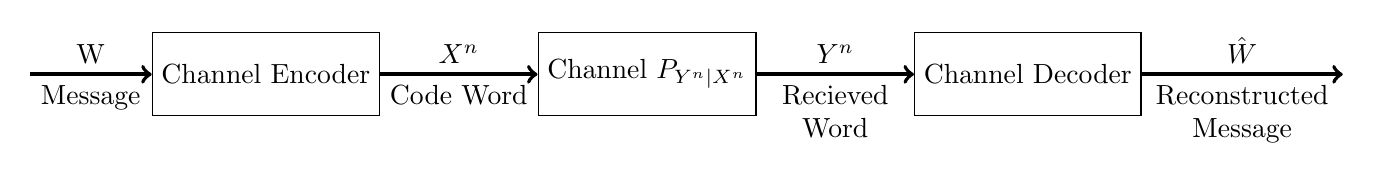
\begin{tikzpicture}
        \node [block] (first) {
            Channel Encoder
        };
        \node [block] [right = 2cm of first] (second) {
            Channel \(P_{Y^n|X^n}\)
        };
        \node [block] [right = 2cm of second] (third) {
            Channel Decoder
        };

        \draw[->, line width = 0.5mm] (first) -- (second) node [pos=0.5, above]{\(X^n\)} node [pos=0.5, below]{Code Word};
        \draw[->, line width = 0.5mm] (second) -- (third) node [pos=0.5, above]{\(Y^n\)} node [pos=0.5, below, align=center]{Recieved \\ Word};
        \draw[->, line width = 0.5mm] +(-3cm, 0) -- (first) node [pos=0.5, above]{W} node [pos=0.5, below]{Message};
        \draw[->, line width = 0.5mm] (third) -- +(4cm, 0) node [pos=0.5, above]{\(\hat{W}\)} node [pos=0.5, below, align=center]{Reconstructed\\Message};
    \end{tikzpicture}
\end{itemize}

\subsubsection{Definitions}
\begin{itemize}
    \item \textbf{Lecture 19 Definition (Discrete Communication Channel): } A discrete communication channel is a triplet
    \[(\mathcal{X}, y, \{P_{Y^n|X^n}\}^\infty_{n=1})\]
    with the following:
    \begin{itemize}
        \item a finite \textit{input} alphabet \(\mathcal{X}\)
        \item a finite \textit{output} alphabet \(\mathcal{Y}\)
        \item a sequence of n-dimensional transition distributions
    \end{itemize}
    \[P_{Y^n|X^n}(b^n|a^n) := P[Y^n=b^n|X^n=a^n]\]
    for \(n\geq1, a^n = (a_1, \ldots, a_n)\in \mathcal{X}^n, b^n = (b_1, \ldots, b_n)\in y^n\), such that \[\sum_{b^n \in y^n} P_{Y^n|X^n} (b^n|a^n) = 1  \ \ \forall a^n \in \mathcal{X}^n\]

    \item \textbf{Lecture 19 Definition (Discrete memoryless channel):} A discrete channel whose sequence of n-dimensional transition distributions satisfy
    \[P_{Y^n|X^n}(b^n|a^n) = \prod_{i=1}^n P_{Y|X}(b_i|a_i)\]
    \(\forall n \geq 1, a^n \in \mathcal{X}^n, b^n \in \mathcal{Y}^n\) 

    \item \textbf{ Lecture 19 Definition (Information Capacity): } Given a DMC \((\mathcal{X}, \mathcal{Y}, Q=[P_{xy}])\), its information capacity C is defined as:
    \[C = \max_{P_X} I(X;Y)\]
    where maximization is over all possible input distributions \(P_X\)
    \item \textbf{Lecture 20 Definition (Symmetric Channels): } A DMC \((\mathcal{X}, \mathcal{Y}, Q=[P_{xy}])\) is called \textit{symmetric} if the rows of Q are permutations of each other and the columns of Q are permutations of each other
    \item \textbf{Lecture 20 Definition (Weakly symmetric channels): } A DMC  \((\mathcal{X}, \mathcal{Y}, Q=[P_{xy}])\) is called \textit{weakly symmetric} if the rows of Q are permutations of each other and all columns sums in Q are equal
    \item \textbf{Lecture 20 Definition (Quasi-Symmetric Channel): } A DMC \((\mathcal{X}, \mathcal{Y}, Q=[P_{xy}])\) is called \textit{quasi-symmetric} if Q can be partitioned along its columns into \textit{weakly symmetric} sub-matricies \(Q_1, \ldots, Q_m\) for some integer \(m \geq 1\) where each sub-matrix \(Q_i\) has size \(|\mathcal{X}| \times |\mathcal{Y}|\) where i = \(1, \ldots, m\)
    with 
    \[y_1 \cup y_2 \cup \cdots \cup y_m = \mathcal{Y} \]
    and 
    \[y_i \cap y_j = \emptyset\]
    \(\forall i \neq j; i,j = 1, \ldots, m \)
    
\end{itemize}
% What does consistent mean??? why is this assumption important?

\subsubsection{Theorems/Lemmas}
\begin{itemize}
    \item \textbf{Lecture 19 Lemma: } The DMC property, 
    \[P_{Y^n|X^n}(b^n|a^n) := P[Y^n=b^n|X^n=a^n]\]
    is equivalent to the following conditions (Both need to be true in order to go backwards)
    \begin{itemize}
        \item \(P_{Y_n|X^n, Y^{n-1}} (b_n|a_n, b^{n-1}) = P_{Y|X} (b_n|a_n) \ \ \forall n \geq 1, a^n \in \mathcal{X}^n, b^n \in \mathcal{Y}^n\)
        \item \(P_{Y^{n-1}|X^n}(b^{n-1}|a^n) = P_{Y^{n-1}|X^{n-1}} (b^{n-1}|a^{n-1}) \ \ \forall n \geq 2, a^n \in \mathcal{X}^n, b^{n-1} \in \mathcal{Y}^{n-1}\)
    \end{itemize}
    \item \textbf{Lecture 20 Lemma: (Information Capacity of weakly symmetric channels): }
    For a \textit{weakly symmetric} DMC \((\mathcal{X}, \mathcal{Y}, Q)\), its information capacity is acheived by a \textit{uniform input distribution} and is given by
    \[C = \log_2|\mathcal{Y}| - H(q_1, q_2, \ldots, q_{|\mathcal{Y}|})\]
    where \((q_1, q_2, \ldots, q_{|\mathcal{Y}|})\) is any row from Q

    \item \textbf{Lecture 20 Lemma (Information Capacity of quasi-symmetric channels): }
    For a \textit{quasi-symmetric} DMC \((\mathcal{X}, \mathcal{Y}, Q=[P_{xy}])\), its information capacity C is acheived by a \textit{uniform input distribution} and is given by
    \[C = \sum_{i=1}^m a_i* C_i\]
    Where 
    \[a_i = \sum_{y \in y_i} P_{xy}\]
    (or sum of any row in \(Q_i\)), and

    \[C_i = \log_2 |y_i| - H(\text{any row in matrix } \frac{1}{a_i} Q_i)\]    
\end{itemize}

\section{Block Codes for Noisy Channels}
\subsubsection{Observations}

\subsubsection{Definitions}
\begin{itemize}
    \item \textbf{Lecture 21 Defintition (Block Codes for Discrete Channels): }
    Given integers n and M, a (n,M) code is for a discrete channel \((\mathcal{X}, \mathcal{Y}, \{P_{Y^n|X^n}\}_{n=1}^\infty)\) with block length n and rate
    \[R_n := \frac{1}{n} \log_2 M\]
    (In message bits per channel symbol) consists of
    \begin{itemize}
        \item A mssage set \(\mu = \{1,2,\ldots, M\}\) intended for transmission
        \item an encoding function
        \[f: \mu \to \mathcal{X}^n\]
        Yielding codewords \(f(1), f(2), \ldots, f(M) \in \mathcal{X}^n\) of length n. The set of codewards is called the codebook:
        \[\mathcal{C}_n = \{f(1), f(2), \ldots, f(M)\}\]
        \item a decoding function
        \[g: \mathcal{Y}^n \to \mu\]
    \end{itemize}
    \item \textbf{Lecture 21 Definition (Average Probability of Error): } Given (n,M) code \(\mathcal{C}_n\), its average probability of error is given by
    \begin{align*}
        P_e & :=P(\hat{W} \neq W) \\
        & = \sum_{w=1}^M P(W=w) P(g(Y^n)\neq w|W=w) \\
        & = \frac{1}{M} \sum_{w=1}^M \lambda_w(\mathcal{C}_n)
    \end{align*}
    Where
    \begin{align*}
        \lambda_w(\mathcal{C}_n)&:= P(g(Y^n) \neq w | W = w) \\
        & = P(g(Y^n)\neq w |X^n = f(w)) \\
        & = \sum_{y^n \in \mathcal{Y}^n: g(y^n) \neq w} P_{Y^n|X^n}(y^n | f(w))
    \end{align*}
    is the code's \textit{contitional probability of decoding error} given that message w is sent over the channel.
    \item \textbf{Lecture 21 Definition (Achievable): } A rate is called achieveable for a discrete channel if there exists a sequence of \((n, M_n)\) block codes \(\mathcal{C}_n\)
    for the channel with
    \[\liminf_{n \to \infty} \frac{1}{n} \log_2 M_n \geq R\]
    and 
    \[\lim_{n \to \infty} P_e(\mathcal{C}_n) = 0\]
    \item \textbf{Lecture 21 Definition (Operational Channel Capacity): } Denoted \(C_{op}\) is defined as follows
    \[C_{op} := \sup \{R: R \text{ is achievable}\}\]

    \item \textbf{Lecture 21 Definition (Jointly typical set): }
    Let \(\{(x_i, y_y)\}_{i=1}^\infty\) be a memoryless source with common pmf \(P_{XY}\) on \(\mathcal{X} \times \mathcal{Y}\). Given \(\delta>0\) and integer \(n\geq 1\), the jointly typical set \(A^{(n)}_\delta\) with respect to the source is
    \begin{align*}
        A^{(n)}_\delta := \{ (x^n, y^n \in \mathcal{X}^n \times \mathcal{Y}^n) :& \big|\frac{-1}{n} \log_2 P_{X^n} (x^n) - H(X)\big| \leq \delta, \\
        & \big|\frac{-1}{n} \log_2 P_{Y^n}(y^n) - H(Y)\big| \leq \delta, \\
        & \big|\frac{-1}{n} \log_2 P_{X^n, Y^n} (x^n, y^n) - H(X,Y)\big| \leq \delta\} \\
    \end{align*}
    \item \textbf{Lecture 24 Definition (Source Channel Block Code):}
    Given a discrete source \(\{V_i\}_{i=1}^\infty\) with alphabet \(\mathcal{V}\) and discrete channel \((\mathcal{X}, \mathcal{Y}, \{P_{Y^n|X^n}\}_{n=1}^\infty)\) an m-to-n source channel block
    code \(\mathcal{C}_{m,n}\) with rate \(\frac{m}{n}\) source symbols per channel symbols is a pair of maps \((f_{sc}, g_{sc})\)
    \[f_{sc}: \mathcal{V}^m \to \mathcal{X}^n\]
    and 
    \[g_{sc}: \mathcal{Y}^n \to \mathcal{V}^m\]

    \item \textbf{Lecture 24 Definition (Code Error Probability):}
    \[P_e(\mathcal{C}_{m,n}):=P(\mathcal{V}^m \neq \hat{V}^m)\]
    %write the rest later

\end{itemize}
\subsubsection{Theorems/Lemmas}
\begin{itemize}
    \item \textbf{Lecture 21 Theorem (Joint AEP):}
    For a DMS \(\{(x_i, y_y)\}_{i=1}^\infty\) with PMF \(P_{XY}\) on \(\mathcal{X} \times \mathcal{Y}\), then the joint typical set \(A^{(n)}_\delta\) satisfies:
    \begin{itemize}
        \item \(P_{X^n,Y^n} (A^{(n)}_\delta) = P((X^n, Y^n) \in A^{(n)}_\delta)> 1 - \delta\) for n sufficiently large
        \item \(|A^{(n)}_\delta| \leq 2^{(H(X,Y) + \delta)} \ \ \ \forall n\)
        \item \(|A^{(n)}_\delta| > (1-\delta) 2^{n*(H(X,Y) - \delta)}\) for n sufficiently large
    \end{itemize}
    \item \textbf{Lecture 22 Theorem (Channel Coding Theorem): }
    For a DMC \((\mathcal{X}, \mathcal{Y}, Q = [P_{XY}])\) with information capacity \(C:= \max_{P_X} I(X;Y)\), its operational capacity, \(C_{op}\) satisfies
    \[C_{op} = C\]
    In other words, the following two results hold
    \begin{itemize}
        \item Forward Part: For any \(0< \epsilon<1\), there exists \(\gamma = \gamma(e)>0\) and a sequence of \((n,M_n)\) block codes \(\mathcal{C}_n\) for the DMC with
        \[\liminf_{n \to \infty} \frac{1}{n} \log_2 M_n \geq C - \gamma\]
        and
        \[P_e(\mathcal{C}_n)< \epsilon\]
        for n sufficiently large
        \item Converse Part: For any sequence of \((n, M_n)\) block codes \(\mathcal{C}_n\) for the DMC with
        \[\liminf_{n \to \infty} \frac{1}{n} \log_2 M_n > C\]
        we have that 
        \[\liminf_{n \to \infty} P_e(\mathcal{C}_n)>0\]
    \end{itemize}
    \item \textbf{Lecture 23 Lemma: } Given a DMC \((\mathcal{X}, \mathcal{Y}, Q = [P_{XY}])\) with arbitrary input word \(X^n\) resulting in output word \(Y^n\), then
    \[I(X^n;Y^n)\leq n * C\]
    where, \(C:= \max_{P_X} I(X;Y)\)

    \item \textbf{Lecture 24 Theorem (Lossless Joint Souce-Channel coding Theorem for Rate-one codes):}
    Given a discrete stationary source \(\{V_i\}_{i=1}^\infty\) with alphabet \(\mathcal{V}\) and entropy rate \(H(\mathcal{V})\) a DMC \((\mathcal{X}, \mathcal{Y}, \{P_{Y^n|X^n}\}_{n=1}^\infty)\) with capacity C, we have:
    \begin{itemize}
        \item \textbf{Forward part (Achievability):} \\
        For any \(0< \epsilon < 1\) and given that the stationary source is also ergodic, if
        \[H(\mathcal{V})<C\]
        then there exists a sequence of rate-one source-channel codes \(\{\mathcal{C}_{m,m}\}_{m=1}^\infty\) with error probability satisfying
        \[P_e(\mathcal{C}_{m,m})<\epsilon\]
        for m sufficiently large
        \item \textbf{Converse Part:} \\
        If 
        \[H(\mathcal{V})>C\]
        then any sequence of rate-one source channel codes \(\{\mathcal{C}_{m,m}\}_{n=1}^\infty\) for the source and channel has error probability satisfying
        \[\liminf_{m \to \infty} P_e(\mathcal{C}_{m,m})>0\]
    \end{itemize}

    \item \textbf{Lecture 24 Theorem (Lossless Join Source-Channel Coding Theorem for General Rates):} 
    Given a discrete stationary source \(\{v_i\}_{i=1}^\infty\) with alphabet \(\mathcal{V}\) and entropy rate \(H(\mathcal{V})\), and a DMC \((\mathcal{X}, \mathcal{Y}, P_{Y|X})\) with capacity C, where
    both \(H(\mathcal{V})\) and X are measured in the same units, then the following hold
    \begin{itemize}
        \item \textbf{Forward Part (Achieveability):} \\
        For any \(0<\epsilon<1\) and given that the stationary source is also ergodic, there exists a sequence of m-to-\(n_m\) source channel codes \(\{\mathcal{C}_{m, n_m}\}_{m=1}^\infty\) with error probability
        \[P_e(\mathcal{C}_{m,n_m})<\epsilon\]
        for m sufficiently large, if
        \[\limsup_{m \to \infty} \frac{m}{n_m}H(\mathcal{V})<C\]
        \item \textbf{Converse Part:} \\
        Any Sequence of m-to-\(n_m\) source-channel codes \(\{\mathcal{C}_{m, n_m}\}_{m=1}^\infty\) for the source and channel with
        \[\limsup_{m \to \infty}\frac{m}{n_m}H(\mathcal{V})>C\]
        has an error probability
        \[\liminf_{m \to \infty} P_e(\mathcal{C}_{m,n_m})>0\]
    \end{itemize}
\end{itemize}
\subsubsection{Observations}
\begin{itemize}
    \item The operational capacity is the largest rate for which there exists a block code where the probability of error goes to zero as block length n approaches infinity.
\end{itemize}

\section{Information theory for continuous alphabet systems}
\subsection{Differential Entropy}
\subsubsection{Definitions}
\begin{itemize}
    \item \textbf{Lecture 25 Definition (Differential Entropy):}
    The differential entropy of a real RV X with PDF \(f_x\) and support \(S_x\) is given by
    \[h(x) := -\int_{S_x}f_x(t)\log_2 f_x(t)dt\]
    and in the multivariate case
    \[h(x^n):=-\int_{S_{x^n}}f_{x^n}(x_1, \ldots, x_n)\log_2 f_{x^n}(x_1, \ldots, x_n)dx_1, \ldots, dx_n\]
    \item \textbf{Lecture 26 Definition (Conditional Differential Entropy):}
    Let \((x,y)~f_{xy}\) with support \(S_{XY} \subseteq \mathbb{R}^2\). The conditional differential entropy of Y given X is given by 
    \[h(y|x) := -\int_{S_{xy}} f_{xy}(x,y) \log_2 f_{y|x}(y|x) dx dy\]

    Chain rule:
    \[h(x,y) = h(x) + h(y|x) = h(y) + h(x|y)\]

    \textbf{Lecture 26 Definition (Divergence):}
    Let X and Y be 2 RVs with pdfs \(f_x \text{ and } f_y\) with supports \(S_X \subseteq S_Y \subseteq \mathbb{R}\)

    \[D(X||Y):= \int_{S_X} f_x(t) \log_2 \frac{f_x(t)}{f_y(t)} dt\]
    Multivariable case:
    \[D(X^n||Y^n) = \int_{S_{X^n}} f_{X^n}(t_1, \ldots, t_n) \log \frac{f_{X^n}(t_1, \ldots, t_n)}{f_{Y^n}(t_1, \ldots, t_n)}dt_1 \ldots dt_n\]

    \item \textbf{Lecture 26 Definition (Differential Cross Entropy):}
    \[h(f_x;f_y) = \int_{S_X} f_x(t) \log_2 \frac{1}{f_y(t)}dt\]
    Note: \(D(f_x||f_y) = -h(f_x) + h(f_x;f_y) \geq 0\)

    \item \textbf{lecture 26 Definition (Mutual Information):}
    \[I(X;Y):= D(f_{xy}||f_x f_y)\]
    \[= h(x) + h(y) - h(x,y)\]

    \item \textbf{Lecture 27 Definition (Multivariate Gaussian):}
    Refer to textbook page 177 for this definition

    \item \textbf{Lecture 28 Definition (Typical Set):}
    For fixed \(\epsilon > 0\) and n,
    \[A_{\epsilon}^{(n)} = \{x^n \in S_{x^n}: |-\frac{1}{n} \log_2 f_{X^n}(X^n) - h(x)| \leq \epsilon\}\]
    \item \textbf{Lecture 28 Definition (Volume):}
    For \(\mathcal{A} \subseteq \mathbb{R}^n\)
    \[vol(\mathbb{R}) = \int_{\mathbb{R}} dx_1, \ldots, dx_n\]
\end{itemize}
\subsubsection{Theorems}
\begin{itemize}
    \item \textbf{Lecture 27 Theorem (Join Differential Entropy of multivariate gaussian):}
    if
    \[\underline{X} = (x_1, \ldots, x_n)^T \sim N(\underline{\mu}, k_{\underline{x}})\]
    then
    \[h(\underline{x}) = \frac{1}{2} \log_2 ((2\pi e)^n \det(k_{\underline{x}}))\]
    \item  Corollary:
    For any real-valued nxn positive-definite matrix \(K=[k_{i,j}]\)
    we have 
    \[\det(K) \leq \prod_{i=1}^{n} k_{i,i}\]
    with equality iff K is a diagonal matrix

    \item \textbf{Lecture 28 Theorem (Maximal Differential Entropy):}
    \[h(\underline{x}) = h(x_1, \ldots, x_n) \leq \frac{1}{2} \log_2((2\pi e)^n \det(K_{\underline{x}}))\]
    with equality iff \(X \sim (\underline{\mu}, K_{\underline{X}})\)
    \item \textbf{Lecture 28 Theorem (AEP for continuous idd RVs):}
    Let \(\{X_i\}_{i=1}^\infty\) be a memoryless real source with PDF \(f_x\) and support \(S_x \subseteq \mathbb{R}\)
    \[-\frac{1}{n} \log_2 f_{X^n}(x_1, \ldots, x_n) \Longrightarrow E[-\log_2 f_x(x)] = h(x)\]
    in probability as \(n \to \infty\)
    \item \textbf{Lecture 28 Theorem (Consequences of the AEP for Continuouse source):}
    \begin{itemize}
        \item \(\lim_{n\to\infty} P_{X^n}(\mathcal{A}_{\epsilon}^{(n)})=1\)
        \item \(Vol(\mathcal{A}_{\epsilon}^{(n)}) \leq 2^{n(h(x)+\epsilon)}\) For all n
        \item \(Vol(\mathcal{A}_{\epsilon}^{(n)}) > (1-\epsilon) 2^{n(h(x)-\epsilon)}\)
    \end{itemize}
\end{itemize}
\subsection{Discrete Time Memoreyless Gaussian Channel}
\subsubsection{Definitions}
\begin{itemize}
    \item \textbf{Discrete-Time Continuous Alphabet Memoryless Channels}
    For a discrete time channel with continuous input and output alphabet, the channel is called memoryless if
    \[f_{Y^n|X^n} (y^n|x^n) = \prod_{i=1}^n f_{Y|X}(y_i|x_i)\]

    In reality, the cost of using the channel is not free. \(b(x)\) is called the cost function and denotes the cost of input \(x\) being sent over the channel and P denotes the budget per input symbol.
    The average cost constraint \((t(*), P)\) requires that on any n-tuple \(x^n = (x_1, \ldots, x_n)\) sent over the channel satisfies
    \[\frac{1}{n} \sum_{i=1}^n t(x_i) \leq P\]

    \item \textbf{Information Capacity with Input Cost:}
    Similar definition in the discrete case. The information capacity of a discrete-time memoryless channel \((\mathcal{X}, \mathcal{Y}, f_{Y|X})\) with input average costraint \((t(*), P)\) is given by
    \[C(P) := \sup_{F_x: E[t(x)]\leq P} I(X;Y)\]
    In other word, the suprememum of mutual information over all input distributions that satisfy the cost contraints.

\end{itemize}
\subsubsection{Theorems/Lemmas}
\begin{itemize}
    \item \textbf{Lecture 29 Lemma (Concavity of C(P) in P):}
    \(C(P)\) is concave, continuous, and increasing in P for \(P>0\)
\end{itemize}
\subsubsection{Observations}
\begin{itemize}
    \item \textbf{Lecture 29:}
    For discrete-time memoryless gaussian channel with noise \(\sigma^2\) and input power constraint \(P\),
    \[C(P) = \frac{1}{2} \log_2(1+\frac{P}{\sigma^2})\]
\end{itemize}

\section{Tutorial Proofs}
\subsection{Week 2 Tutorial}
\begin{itemize}
    \item Given 2 discrete RVs, \(X, Y\) we have that
    \[H(Y|X) = 0 \Longleftrightarrow \text{Y is a function of X}\]
    \item Given RV \(X\) with alphabet \(\mathcal{X}\) and function \(f: x \to \mathbb{R}\)
    \[H(X) \leq H(f(X))\]
\end{itemize}
\subsection{Week 3 Tutorial}

% Random helpful links
% https://math.stackexchange.com/questions/4531722/simplifying-entropy-hx-y-xy
% https://pysdr.org/content/channel_coding.html
% https://math.stackexchange.com/questions/4547648/prove-ab-log-2ab-leq-a-log-2a-b-log-2b


\end{document}
